\chapter{特征表示的底层语义应用}
\label{chap:Denoising}


\section{图像的去噪方法}
图像去噪的目的是从噪声图像中恢复出原图像,这是低级视觉任务中的一个经典问题。由于无噪声的原图像通常是未知的,因此这个问题本质上是不适定的,即它是一个欠定的映射问题,通常映射变换不唯一。一般来说,残差图像$ F $可以表示为$ F = y-f(x)$,其中$ x $是噪声图像,$ f $是映射函数,它接收输入图像并将其转换为输出图像。$ y $是理想的无噪声图像。通过应用不同类型的映射函数,相同的数学模型适用于大多数其他低层级的视觉图像任务,如图像去模糊,去马赛克和超分辨率等。

最近,无论是从高级到低级视觉任务,深度神经网络在计算机视觉领域表现出了卓越的性能。众所周知,神经网络能够将任何可测量的函数逼近到期望的准确度\cite{Hornik1989}。在图像去噪场景下,回归框架中的神经网络试图在某些输入噪声分布下逼近潜在条件期望。当以监督方式训练前馈神经网络时,一个关键因素是选择损失函数来测量输出和真实图像之间的差异。最广泛使用的是像素损失,其通过失真图像和参考图像像素的强度差异以及相关的峰值信噪比\cite{Wang2004}来计算。但是,像素损失不能捕捉到感知差异,并且与人类感知图像质量的关联性很差\cite{Zhao2015,Zhanga2012}。这是因为当使用像素损失时隐含地做出的许多假设不能被满足-其主要仅依据于图像的局部灰度特征来处理噪声;相反,人类视觉系统对噪声的敏感性取决于局部亮度,对比度和结构等综合因素\citep{Wang2004}。

基于纯粹的学习策略,为图像去噪设计一组深度神经网络已被证明优于其他被广泛采用的传统方法\cite{Burger2012}。但是,所有这些基于学习策略的工作都存在一个问题:如果输入无噪图像,则学习到的模型仍会降低并没噪声的原图像的质量。所以他们工作就是必须限定在给定噪声水平下才有效。用于去除噪声的通用标准算法应该能够处理不同级别的噪声水平,针对具体不同噪声水平需要一系列网络,通常这是不切实际的,甚至是不现实的,因为我们不知道真实图像具体的噪声水平和类型。

我们的主要贡献简要概述如下:
\begin{enumerate}
\item 我们提出了一个深层的全卷积网络结构,用于学习图像残差,针对图像变换对残差映射函数进行建模,直接学习噪声分布。
\item 通过对比像素和感知损失函数的优缺点,训练具有融合底层和高层特征表示信息的变换网络,高效地得到高质量的去噪图像。
\item 为使单个神经网络适用于不同噪声水平,基于网络的统计概率估计,对输入不添加噪声,迫使学习到的网络模型对干净的图像不再进行降级处理;添加不同噪声水平的随机噪声送入网络使得网络模型能针对所有噪声水平进行去噪。
\item 在基准数据集上进行详尽实验,结果表明所采用的新型损失层改进了当前仅基于像素损失的去噪方法。
\end{enumerate}

\subsection{相关工作}
针对图像去噪当前已经提出了相当多的方法,一些方法有选择地平滑噪声图像的部分区域,目的是在保留图像细节的同时“平滑”噪声。一些方法将图像信号变换到可以容易地从信号中分离出噪声的变换 域。最近一些方法利用图像的“非局部”统计:基于相同图像中的不同区域在外观上通常相似的假设,提出块匹配的3D滤波(BM3D)算法\cite{Dabov2007},通过协作滤波在变换域中对非局部相似区域块进行分组,BM3D已经成为自然图像去噪的基准测试方法。

虽然手工设计的BM3D是一种高效算法,但基于学习的方法已经广泛用于图像去噪。神经网络方法和其他去噪方法最显著的区别在于,它们通常自动直接从带噪声图像中学习图像变换,而不是依赖人类先验。最近,由于深度神经网络的快速发展,许多新型的神经网络已经应用于图像去噪问题,如堆叠式稀疏自动编码器\cite{Vincent2008,Xie2012,Agostinelli2013,Technologii2013a,Skribtsov2016},多层感知器\cite{Burger2012,Wang2014a},深度卷积网络\cite{Jain2009,Wu2014,Zhao2015,Mao2016,Eigen2013,Wu2014relu,Wang2015g}。

堆叠式自动编码器\cite{Vincent2008}建立了使用去噪标准作为无监督目标的代价函数,以指导学习高层次语义级别的特征表示。去噪性能可以很容易地测量和直接优化。但是这种方法的目标是分类,Xie等人\cite{Xie2012}提出了一种替代的监督训练方案-堆叠式稀疏降噪自动编码器,该方法将稀疏编码和深度网络结合起来,用去噪自动编码器进行预训练,成功地将最初设计用于无监督特征学习的自动编码器,变为适用于图像去噪和缺失自动补全任务。

Burger等\cite{Burger2012}提出了一种基于具有普通多层感知器去噪算法,通过在大型数据集上训练学习,其性能优于BM3D。然而,他们的方法适合于特定水平的噪声,并不能很好地推广到其他噪声水平。Jain等人\cite{Jain2009}提出了结合深度卷积神经网络和无监督学习过程,发现卷积网络比基于小波和马尔科夫随机场方法具有更好的去噪性能。

迄今为止,通过在大数据集上训练具有像素损失函数的深度神经网络用于图像去噪任务,但可能会遭受一般性问题,即像素损失与感知图像质量的相关性很低\cite{Zhao2015}。最近有论文已经在图像生成领域,使用感知损失来优化感知目标的图像的质量,其取决于从卷积网络提取的高级特征之间的伽马矩阵的相似性\cite{Dosovitskiy2016}。文献\citepns{Johnson2016,Mao2016}的工作与我们的工作特别相关,其训练前馈神经网络以学习图像变换,使用预先训练用于图像分类的损失网络来定义感知损失函数,以测量输出和真实标签的感知差异。不过他们专注于风格转换和图像超分辨率。我们的网络应用具有编码器-解码器结构的卷积和反卷积层,并且使用对称跳跃连接来加速收敛速度,图像的噪声通过卷积来捕获,并通过解卷积来恢复无噪声图像的细节,可以看作是学习具有对称跳跃连接的变换函数。

Zhao等人\cite{Zhao2015}研究了包括感知损失在内的多种损失的表现,并提出了一种新颖的可微分误差函数,从感知目标设计出一些新的损失层。Wang等人\cite{Wang2014a}也与我们的研究特别相关,他们研究了自然图像块在线性变换方面的分布不变性,他们展示了如何使一个现有的深度神经网络学习多级别的高斯噪声分布。然而,与上述方法不同,本文通过训练具有感知损失函数的前馈变换网络,基于学习优化的图像变换方法,同时通过显式训练不同级别的噪声并使原始图像同样作为输入,使单个深度神经网络在不同级别的加性高斯白噪声下工作良好。

\subsection{提出的方法} 

\label{sec:method}
\begin{figure*}
\vspace{-6mm}
\centering
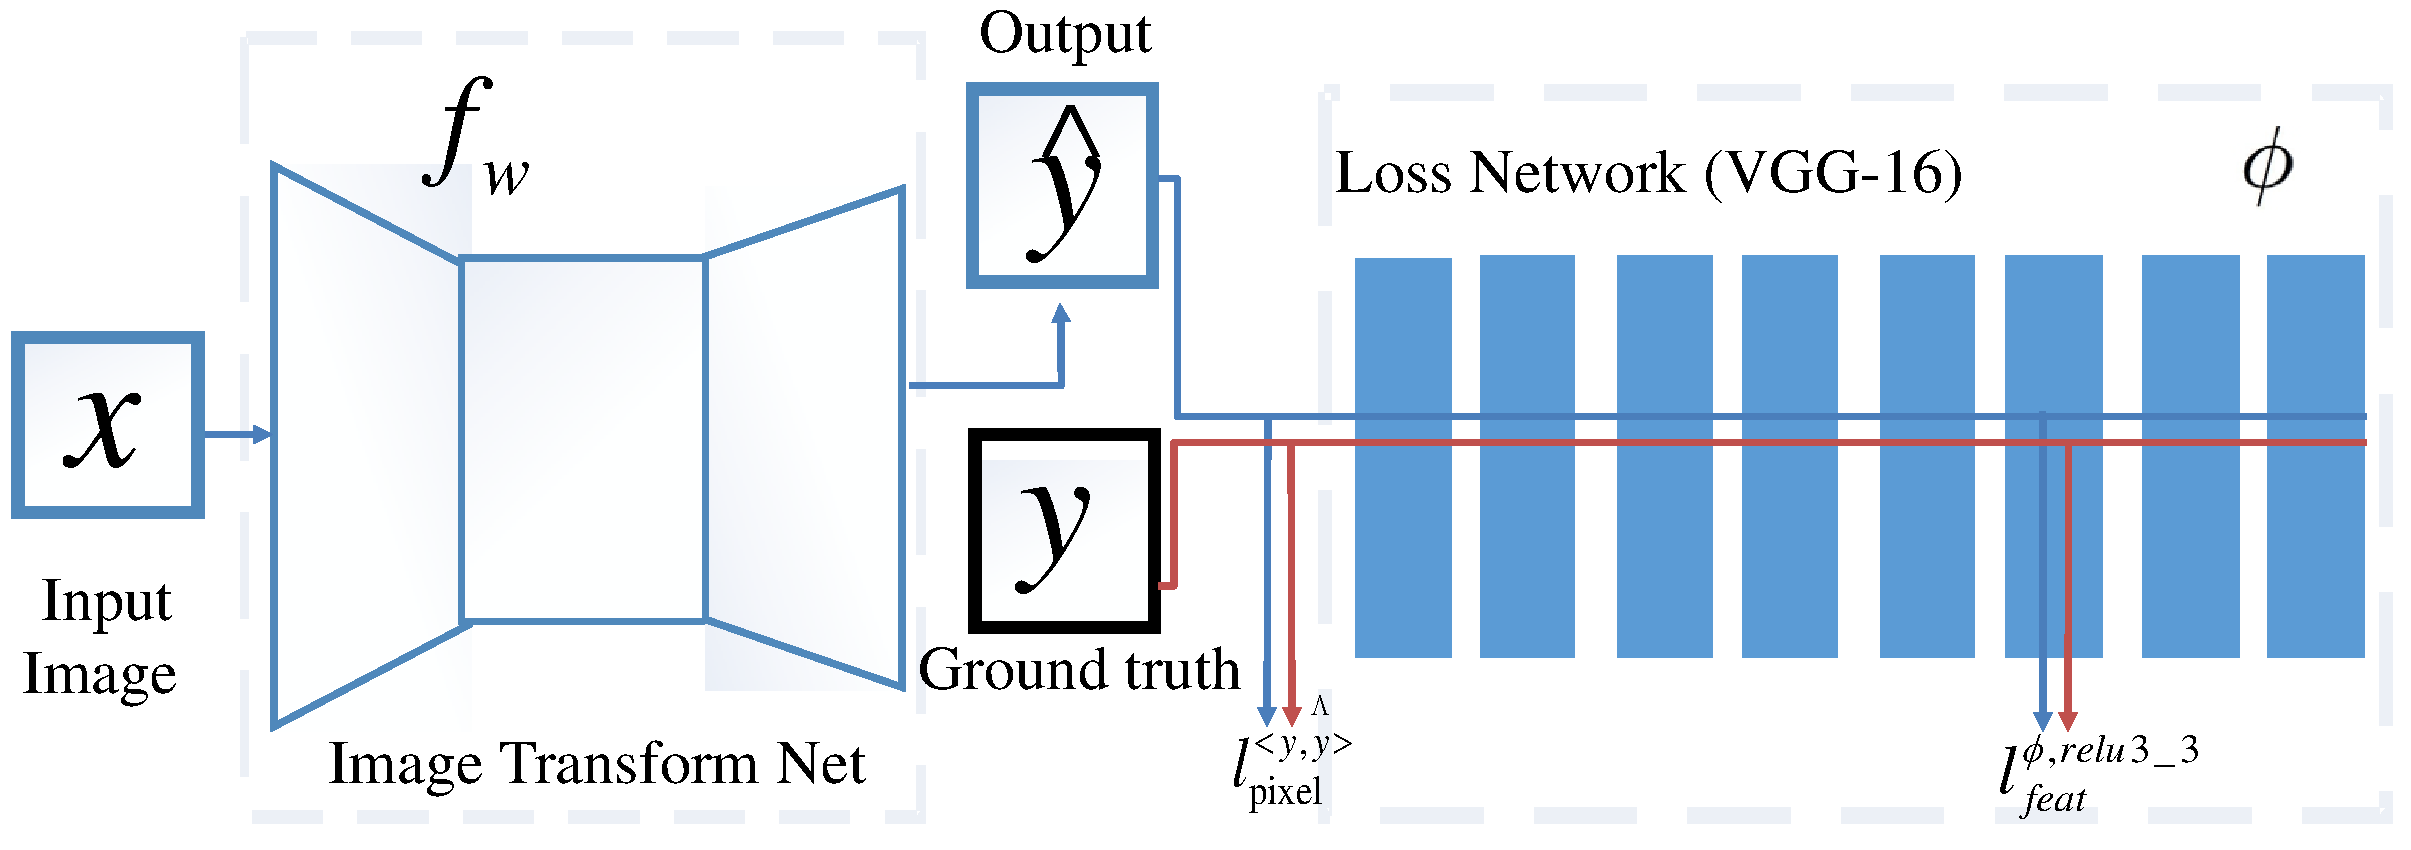
\includegraphics[width=0.9\textwidth]{ch06_01}
\caption[提出网络的整体架构图]{提出的网络的整体架构示意图。图像变换网络包含卷积(编码器)和解卷积(解码器)层。我们使用预先训练的图像分类的损失网络的特征表示来定义感知损失函数,这些函数测量输出和真实标签的感知差异,损失网络的特征表示在训练过程中保持不变。}
\label{fig:ch06_01}
\vspace{-2mm}
\end{figure*}
 
所提出的框架主要包含一系列卷积层和反卷积层,如图\ref{fig:ch06_01}所示。它由两部分组成:一个\emph {图像转换网络} $ f_W $和一个\emph{损失网络} $ \phi $,用于定义几个\emph {代价损失函数} $ \ell_1,\ldots,\ell_k$。旨在学习由权重$ W $参数化的深度残差卷积神经网络; 它通过映射$ \hat y = f_W (x)$将输入图像$ x $转换成输出图像$ f_W $。
每个损失函数计算标量值$ \ell_i(\hat y,y_i)$,测量输出图像$ \hat y $和 \emph{目标图像} $ y_i $之间的差异。学习目标是使用随机梯度下降来训练以最小化损失函数的加权组合:
\begin{equation}
   W^* = \arg\min_W E_{x, \{y_i\}}\begin{bmatrix}
\sum_{i=1} \lambda_i \ell_i(f_W(x), y_i)
\end{bmatrix}
\end{equation}

从这个公式中,我们可以看到优化算法的任务是找到最接近图像变换的映射函数$ f_W $。同时我们也希望$ f_W(y_i)$近似于图像$ y_i $,所以我们现在通过在不同情况下选择合适的权重$ W $来将图像去噪问题统一在一个统一的框架中。损失网络$ \phi $用于定义一个\emph{特征空间损失} $ \ell_{feat}^\phi $和一个\emph{像素损失} $ \ell_{mse} $。对于图像去噪,输入图像$ x $是一个有噪声的输入,真实图像$ y $是目标图像。
  
\begin{figure}[t]
\centering
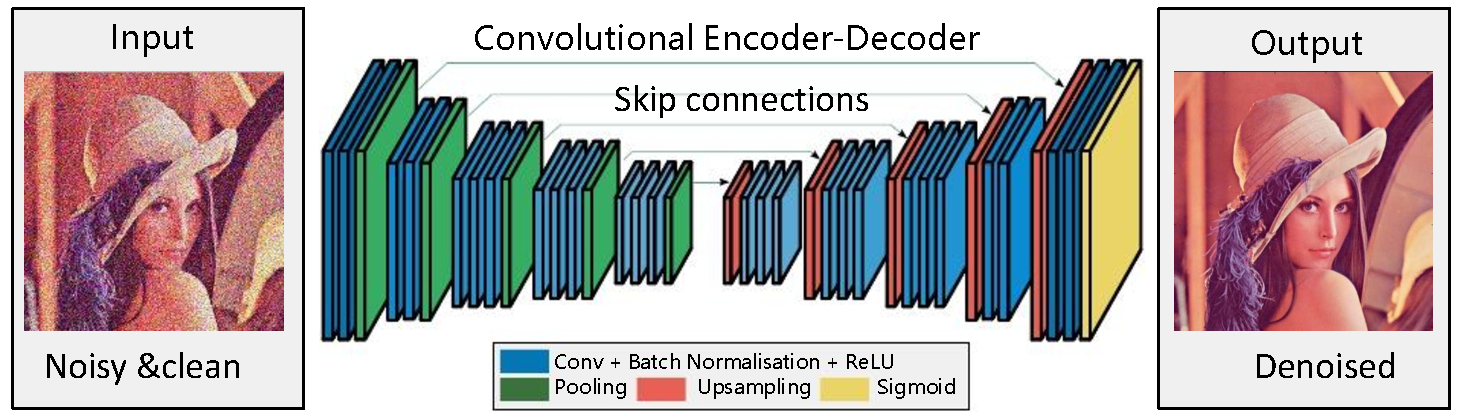
\includegraphics[width=0.9\textwidth]{ch06_02}
\caption{ RED-NET的网络结构示意图}
\label{fig:ch06_02}
\vspace{-6mm}
\end{figure} 
\subsubsection{编码器-解码器卷积结构}

该框架完全是编码器-解码器卷积模型,NohH等\cite{NohH2015,hong2015decoupled,Long2017Fully,Dong2016,Mao2016}已经提出了用于无监督和有监督深度学习的编码器-解码器的神经网络。

我们的图像转换网络大致遵循\cite{Mao2016}提出的网络架构RED-NET用于图像去噪,网络结构如图\ref{fig:ch06_02}所示。基于该网络结构,在卷积之后添加批量归一化\cite{Ioffe2014Batch}和ReLU非线性层;并在网络中插入一些残差网络的模块\cite{he15},输出层使用sigmoid函数来确保输出图像的像素范围为$[0,1]$之间,但是我们不使用任何池化层降低分辨率,而是使用不同步长卷积来进行下采样和上采样。除了第一层和最后一层使用$9\times 9$的卷积核之外,所有卷积层都使用$3 \times 3$的卷积核。由于图像变换网络是完全卷积的,因此在测试时它们可以应用于任何尺寸的图像输入。

RED-NET和我们的去噪网络(DeNET)的区别在于我们的网络插入了一些残差模块块并在不同模块间引入了跳跃连接。在图像去噪的过程中,图像内容的细节可以通过感知损失函数进行补偿,两个网络的具体参数配置在表 \ref{table1}中描述。

将两种学习策略应用于编解码网络的内部模块以使训练更有效,跳跃连接每两个卷积层传递到它们的镜像解卷积层。He等\cite{he15}使用残差连接来训练非常深的网络进行图像分类,他们认为残差连接使网络很容易学习具有很多层的网络模型(如152层);这对于底层任务的图像变换网络来说是一个吸引人的特性,因为在大多数情况下,输出图像应该与输入图像共享大部分内容结构。因此,我们网络的主体由多个残差块组成,每个残块包含两个$ 3\times 3 $大小卷积核的卷积层。
 
\begin{table}
\vspace{-4mm}
\centering
\caption[DeNET-R和RED-NET网络的配置参数表]{DeNET-R和RED-NET网络的参数配置。“conv3”和“deconv3”代表大小为$ 3 \times3 $的卷积和反卷积核。32,128和512是每个卷积和反卷积之后的特征映射的数量。“$ c $”是输入和输出图像的通道数量。}
\begin{tabular}{l | l }\hline
DeNET-R                   &RED-NET                \\ \hline
(conv9-32)$\times$6             &(conv3-128)$\times$6       \\ \hline
(conv3-64)$\times$6             &(conv3-256)$\times$6       \\ \hline
(conv3-128)$\times$3             &(conv3-512)$\times$3       \\ \hline
Residual block$\times$5 &                           \\ \hline
(deconv3-64)$\times$2           &(deconv3-512)$\times$2       \\ \hline
(deconv3-32)$\times$6           &(deconv3-512)$\times$6       \\ \hline
(deconv9-3) $\times$6           &(deconv3-512)$\times$6       \\ \hline
(deconv3-$c$)           &(deconv3-$c$)                \\ \hline
\end{tabular}
\label{table1}
%\vspace{-15mm}
\end{table}
\subsubsection{像素损失函数}
\emph{像素损失}是目标$ \hat y $和输出图像$ y $之间的(归一化)欧几里德距离。若二者大小为$ C \times H \times W $,那么像素欧几里得损失定义为均方误差(MSE):
 \begin{equation}
   \ell_2(\hat y, y) = \frac{1}{CHW}\|\hat y - y\|_2^2
  \end{equation}

这种损失函数可能会引入网格棋盘效应,因此可引入了\lone 范数正则化损失加以缓解。这两种损失对像素错误的权衡是不同的:\lone 不会过度惩罚更大的错误值,因此它们可能具有不同的收敛性质,计算\lone 损失很简单:
\begin{equation}
\ell_1(\hat y, y) = \frac{1}{CHW}| \hat y - y|
\end{equation}
其应用反向传播的求导也是很简单的, 对整个图像的每一像素 $p$来说,
\begin{equation}
\partial \ell_1/\partial p  = sign\left(\hat y(p) - y(p)\right)
\end{equation}
其中,在整个图像上计算$ \ell_1 $的导数将针对图像中的每个像素进行反向传播。

\subsubsection{感知损失函数}

为了测量图像之间感知语义差异提出\emph{感知损失函数},跟文献\citepns{Zhao2015}中提出的手工设计结构相似性(SSIM)损失不同,可利用用于图像分类的预先训练网络作为\emph{损失网络} $ \phi $。在我们所有的实验中,$ \phi $都是16层VGG网络\cite{Simonyan2014a},其是在ImageNet数据集\cite{Deng2009ImageNet}上预先训练的。并不是鼓励输出图像$ \hat y = f_W(x)$的像素完全匹配目标图像$ y $的像素,而是鼓励它们具有由损失网络$ \phi $定义计算的相似特征表示。让$ \phi_j(x)$为图像$ x $的第$ j $层卷积网络$ \phi $的激活值; 然后$ \phi_j(x)$将是卷积层形状大小为$ C_j \times H_j \times W_j $的特征映射。\emph{特征表示损失}是特征表示之间的(归一化平方和)欧几里得距离: 
\begin{equation}
  \ell_{feat}^{\phi,j}(\hat y, y) = 
  \frac1{C_jH_jW_j}\|\phi_j(\hat y) - \phi_j(y)\|_2^2
\end{equation}
欧几里德距离又称为$ \ell_{2} $ 范数距离,如文献\citepns{Mahendran2015}中指出最小化网络初级特征相似性,可以寻找生成图像$ \hat y $,往往会产生与$ y $一致的图像。使用特征损失来训练我们的图像转换网络输出图像$ \hat y $与感兴趣的图像$ y $相似,但不会强制它们完全匹配。为了鼓励输出图像$ \hat y $的空间平滑度,遵循之前关于特征重建\cite{Mahendran2015}的工作,并使用\emph {变分正则化损失函数} $ \ell_{TV}(\hat y)$。
 
\subsection{实验结果分析和讨论}
\label{sec:experiments-results}

在本节中,使用编码器-解码器的卷积神经网络对我们各种实验设置进行分析,然后评估我们的模型在一些不同的损失函数组合设置下的去噪性能。最后,我们探讨如何让一个神经网络处理不同程度的噪声。
\subsection{详尽分析模型}

\begin{table}[b]\label{tab:Denoising-results}  
\vspace{-2mm} 
\footnotesize% fontsize
   \centering{
   \caption{{\it Set14}上的单一噪声水平的图像去噪结果定量比较表}
   \scalebox{0.75}{
     \begin{tabular}{|c|c|c|c|c|c|c|}
       \hline
        \multirow{2}{*}{Sigma} & Noisy & RED-NET\cite{Mao2016} & Ours ($\ell_{2})$ & Ours ($\ell_{1}$)& Ours ($\ell_{feat}$) & Ours ($\ell_{mix}$)\\
   & PSNR / SSIM & PSNR / SSIM & PSNR / SSIM & PSNR / SSIM & PSNR / SSIM & PSNR / SSIM\\
   \hline
    \multirow{1}{*}{$\sigma=10$} & 28.16 / 0.7041 & \textbf{34.81} / \textbf{0.9402}
           & 34.35 / 0.8912 & 33.40 / 0.8930& 31.05 / 0.7680& 33.16 / 0.7680  \\
          % \hline 
    \multirow{1}{*}{$\sigma=30$} & 18.88 / 0.3389 & 29.17 / 0.8423
           & 28.73 / 0.8205 & 29.76 / 0.991& 26.70 / 0.6845& \textbf{30.15} / \textbf{0.8681}  \\
          % \hline
    \multirow{1}{*}{$\sigma=50$} & 14.79 / 0.2038 & 26.81 / 0.7733
           & 26.40 / 0.8205 & 26.79 / \textbf{0.8325}& 25.69 / 0.6411& \textbf{27.09} / 0.8312  \\
          % \hline
    \multirow{1}{*}{$\sigma=70$} & 12.43 / 0.1391 & 25.31 / 0.7206
           & 25.39 / 0.7105 & 26.13 / \textbf{0.7250}& 17.89 / 0.6650& \textbf{26.20} / 0.7180  \\
    \multirow{1}{*}{$\sigma=100$} & 10.26 / 0.0901 &  -
           & 18.40 / 0.4215 & 20.17 / 0.4680& 17.31 / 0.3640& \textbf{19.16} / \textbf{0.4695}  \\
           \hline
        
\end{tabular} 
}}  
\vspace{-4mm}
\end{table}
我们通过同时最小化多个损失函数:$ \ell_{2} $-均方误差(MSE)损失,$ \ell_{1} $-范数损失和特征损失,在具有不同标准偏差$ \sigma $的噪声图像对来训练模型。训练集中图像大小为$ 256 \times 256 $,并通过添加$ \sigma $大小的高斯噪声生成带噪声和无噪声图像对,使用Adam\cite{Kingma2014Adam}的自适应优化算法进行批随机梯度下降算法进行训练,学习速度为$1 \times 10^{-3}$,不使用权重衰减或Dropout等正则化技术。

去噪实验在14个三通道彩色图像的通用基准测试图像{\it Set14}上执行,将零均值和标准差$ \sigma $的加性高斯噪声添加到测试图像中,以测试去噪方法的性能,评价指标选取参考文献\citep{Mao2016,Zhao2015}中的峰值信噪比(PSNR)和结构相似性度量(SSIM)\cite{Wang2004}。

作为基准模型,我们使用RED-NET\cite{Mao2016}作为比较对象,它是一个全卷积网络,具有卷积和反卷积层,损失函数为像素损失。为了说明RED-NET和我们的模型在数据,训练和网络结构方面的差异,我们使用$ \ell_{2} $对相同的标准偏差$ \sigma $进行图像变换网络训练,在使用像素损失的基础上进行消融实验,添加特征损失函数(见Section\ref{sec:method}),以允许从预训损失网络传输语义知识作为有监督的信号指导去噪的去噪网络。

\begin{figure}[t]
\centering
  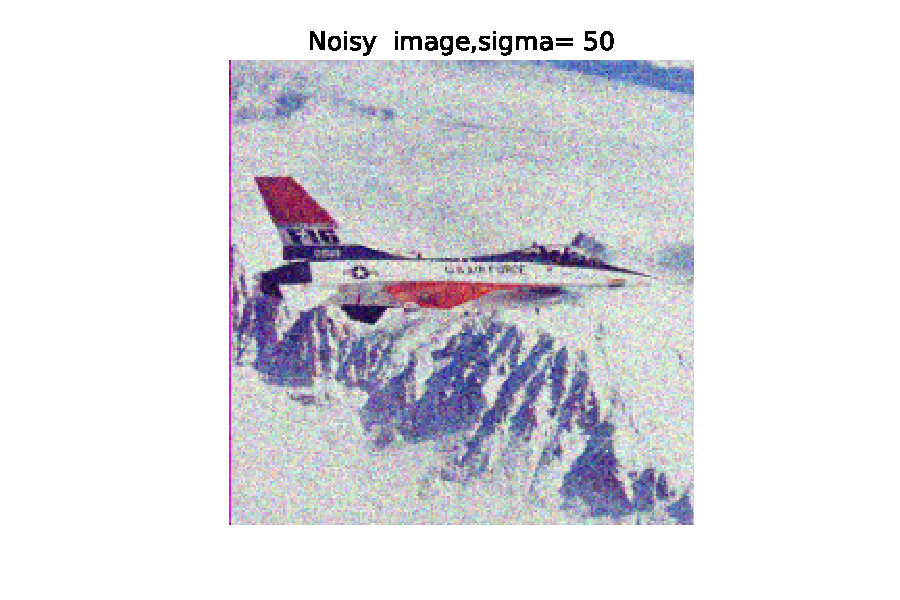
\includegraphics[width=0.17\textwidth]{figs/loss/noisy.pdf}
  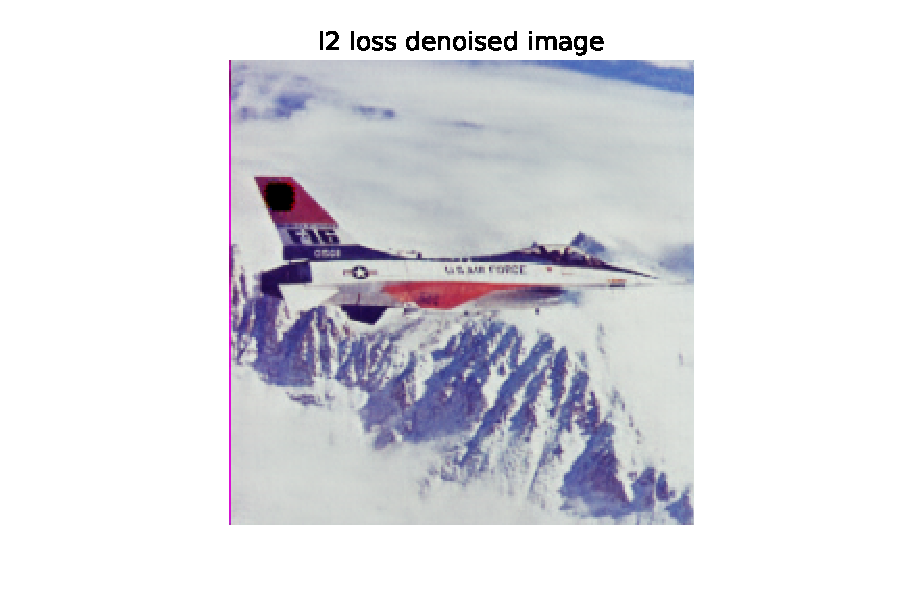
\includegraphics[width=0.17\textwidth]{figs/loss/l2.pdf}
  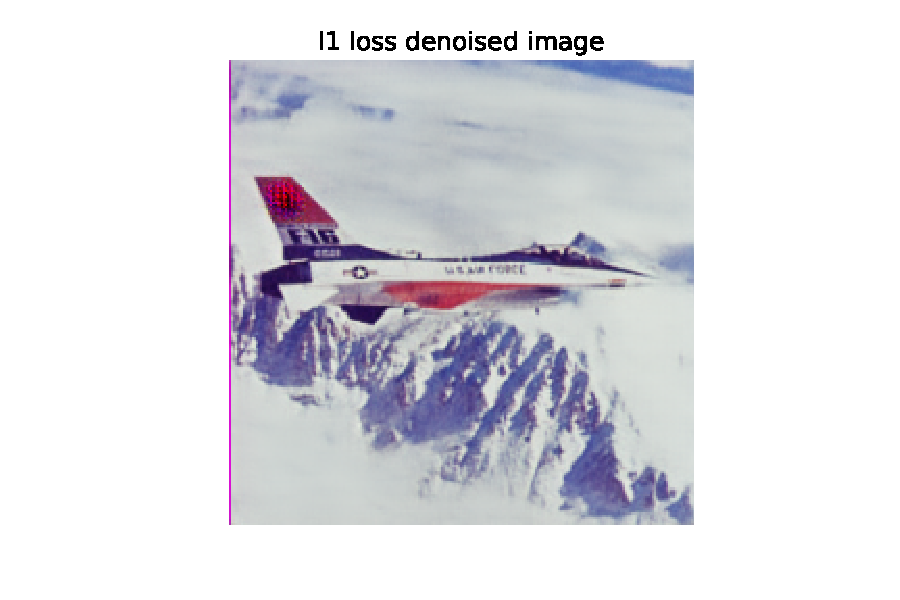
\includegraphics[width=0.17\textwidth]{figs/loss/l1.pdf}
  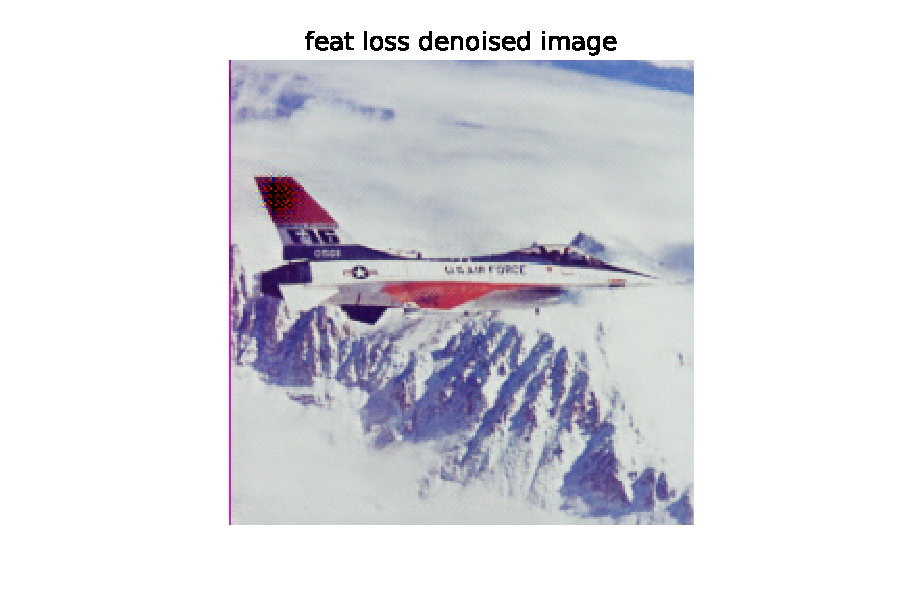
\includegraphics[width=0.17\textwidth]{figs/loss/feat.pdf}
  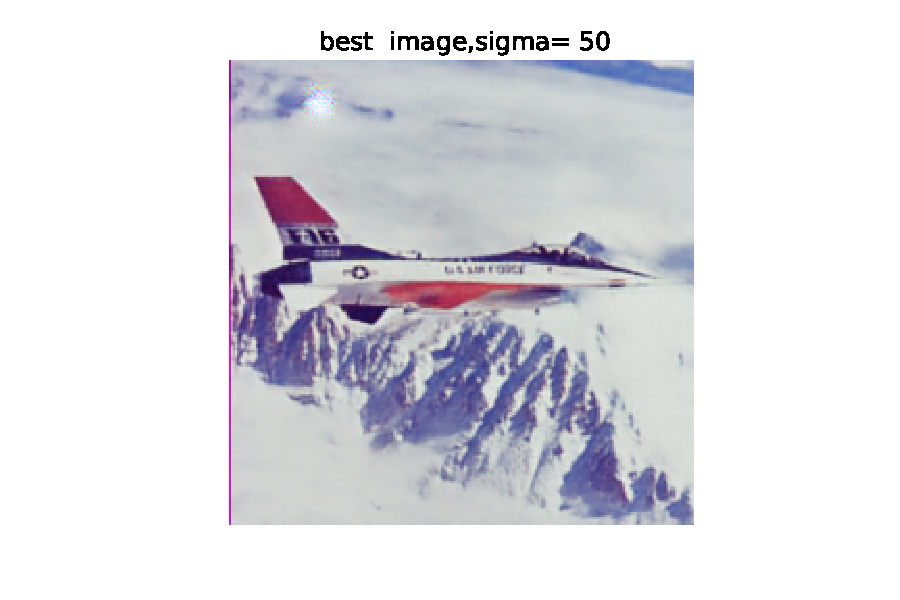
\includegraphics[width=0.17\textwidth]{figs/loss/mix.pdf}  \\{}
  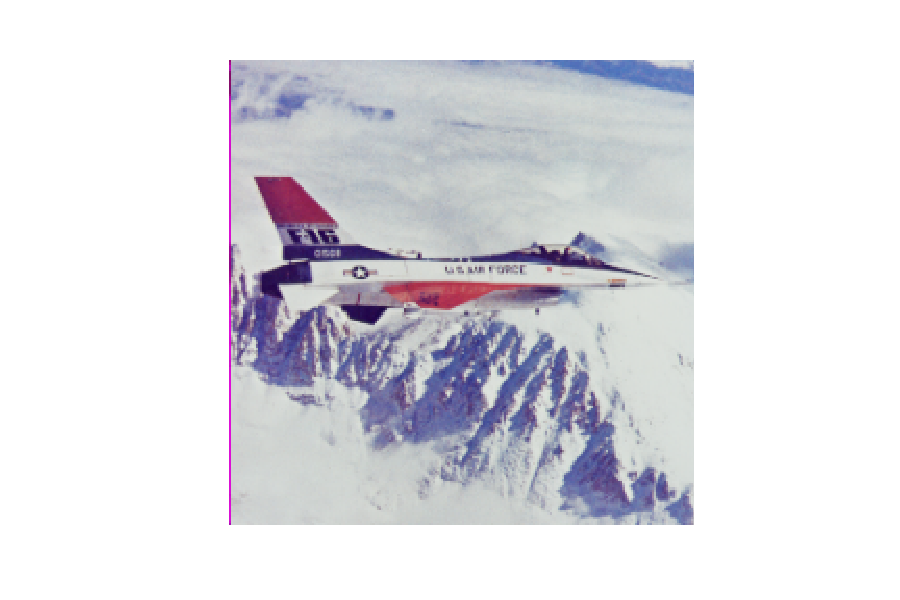
\includegraphics[trim={15pt 60pt 15pt 62pt},width=0.17\textwidth,clip]{figs/loss/orign.pdf}
  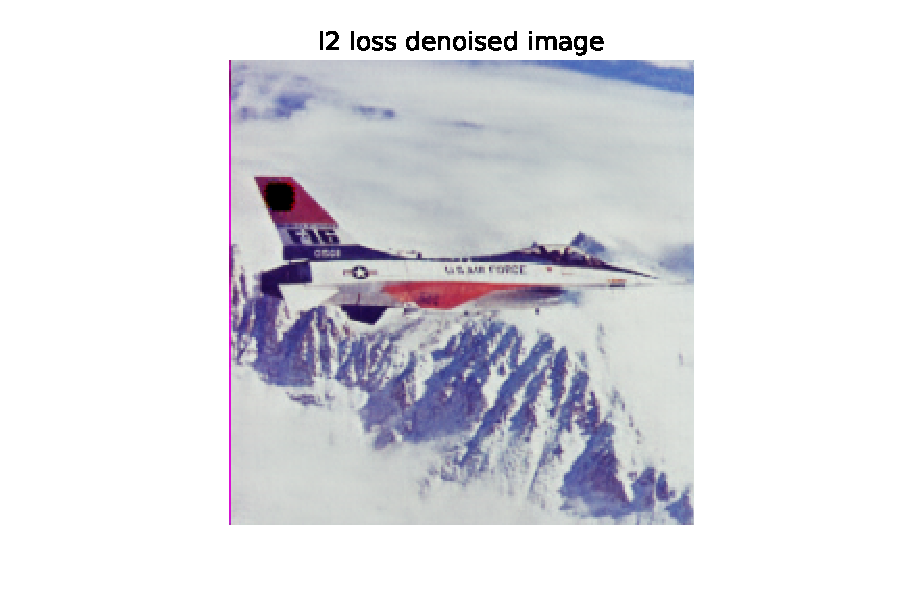
\includegraphics[trim={15pt 60pt 15pt 75pt},width=0.17\textwidth,clip]{figs/loss/l2.pdf}
  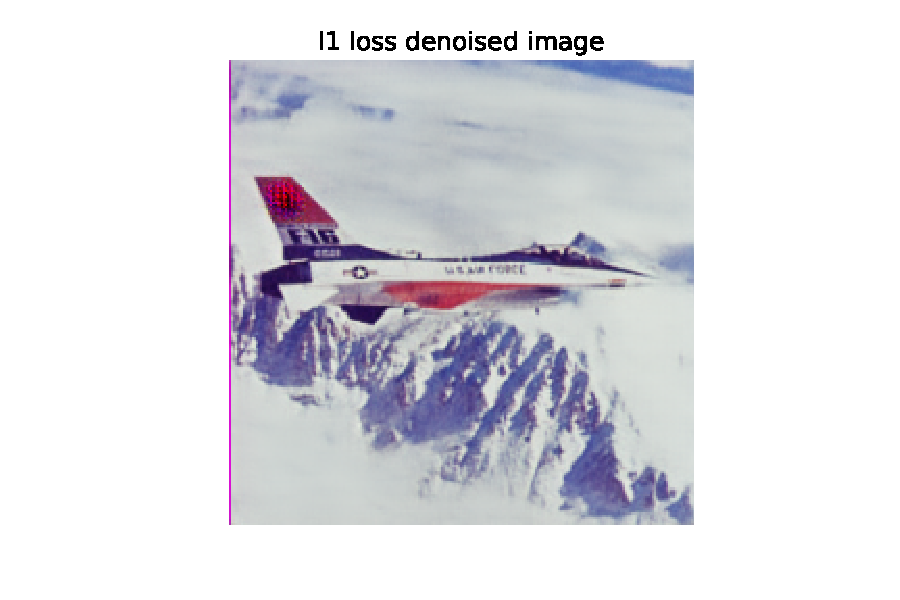
\includegraphics[trim={15pt 60pt 15pt 75pt},width=0.17\textwidth,clip]{figs/loss/l1.pdf}
  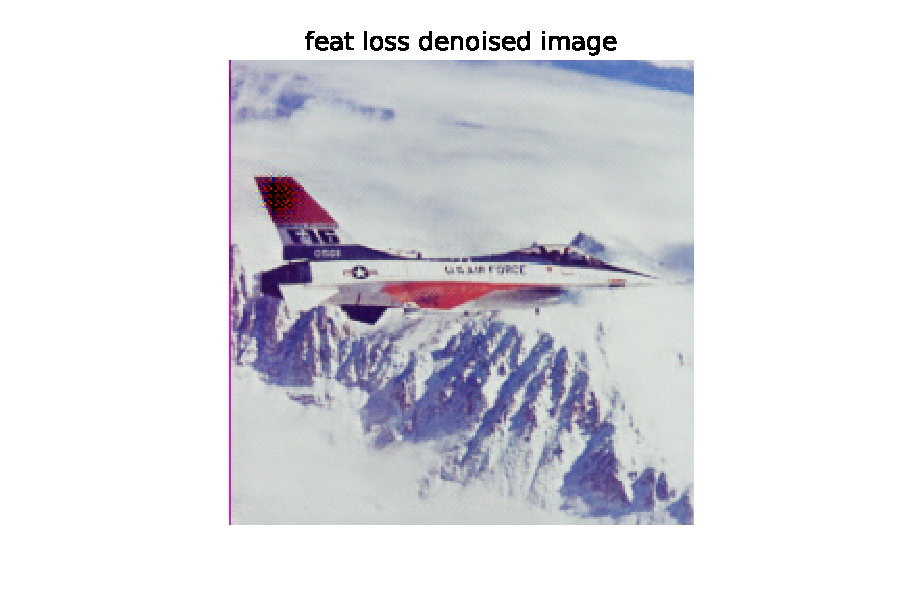
\includegraphics[trim={15pt 60pt 15pt 75pt},width=0.17\textwidth,clip]{figs/loss/feat.pdf}
  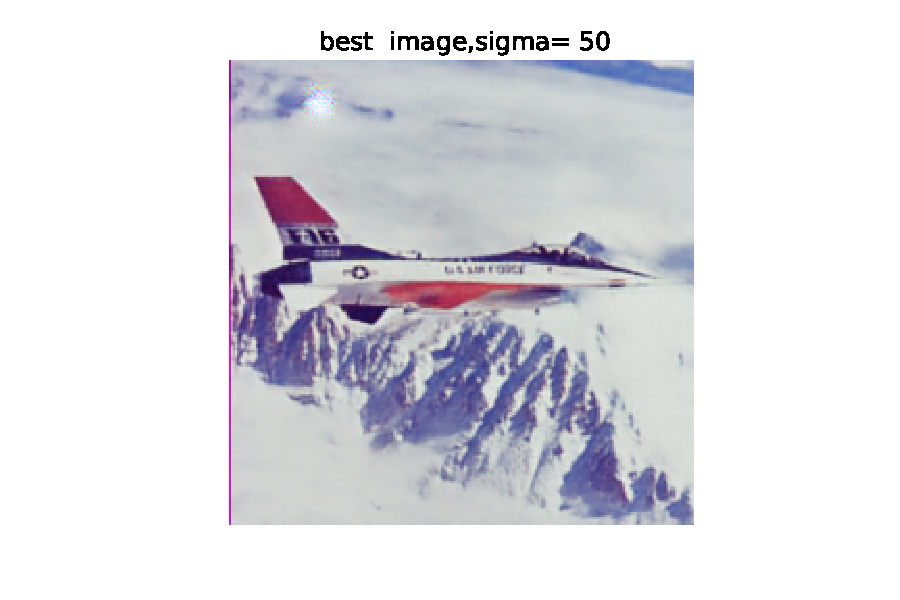
\includegraphics[trim={15pt 60pt 15pt 75pt},width=0.17\textwidth,clip]{figs/loss/mix.pdf} \\
   \begin{minipage}{0.17\textwidth}
        \centering \textbf{Ground Truth} \\ PSNR / SSIM
   \end{minipage}
   \begin{minipage}{0.17\textwidth}
     \centering \textbf{Ours}($\ell_{2}$) \\ 29.11 / 0.8833
   \end{minipage}
   \begin{minipage}{0.17\textwidth}
     \centering \textbf{Ours} ($\ell_{1}$) \\ 29.27 / 0.8841
   \end{minipage}
   \begin{minipage}{0.17\textwidth}
     \centering \textbf{Ours} ($\ell_{feat}$) \\  19.61 / 0.6560
   \end{minipage}
   \begin{minipage}{0.17\textwidth}
     \centering \textbf{Ours} ($\ell_{mix}$) \\  29.31 / 0.8946
   \end{minipage} \\
  \caption[不同损失在基准数据集上的定量比较结果表]{不同损失在基准数据集上的定量比较结果表,在来自{\it Set14}数据集的图像上以不同的损失类型去噪结果。 我们以F-16图像的PSNR / SSIM为例。 
  }
  \vspace{-4mm}
  \label{fig:l1-l2-feat-results}
\end{figure}
首先,与像素损失$ \ell_{1} $和$ \ell_{2} $结果相比,$ \ell_{1} $在去噪性能方面做得更好,同时还原了锐利的边缘和细节,但存在网格棋盘效应。如图\ref{fig:l1-l2-feat-results}所示,
$ \ell_{2} $图像中的机翼以及$ \ell_{2} $图像中的主体的红色块元素。这是因为$ \ell_{2} $惩罚更大的错误值,无论图像中的底层结构如何,都会产生小的错误,其结论与文献{Zhao2015}一致。

此外,若只有特征损失时,在放大数倍分辨率下才能看到轻微的网格棋盘效应,结果为$ \ell_{feat} $如图\ref{fig:l1-l2-feat-results}所示,与基准方法相比,会损害其PSNR和SSIM。我们再次看到,与其他方法相比,我们的$ \ell_{feat} $模型在边缘和细节方面做得很好,比如机翼。$ \ell_{feat} $损失不会不加区分地锐化,与$ \ell_{pixel} $损失相比,$ \ell_{feat} $损失锐化了机翼和骑手的边界边缘,但背景仍然是漫反射的,这表明$ \ell_{feat} $损失可能是更了解图像语义。

由于采用的$ \ell_{pixel} $和$ \ell_{feat} $损失共享相同的架构,数据和训练过程,它们之间的所有差异都是由于$ \ell_{pixel} $和$ \ell_{feat} $损失。$ \ell_{pixel} $损失产生较少的视觉伪像和较高的PSNR值,但$ \ell_{feat} $损失在重建细节方面做得更好,从而导致令人满意的视觉效果。

最后,我们可以观察到单个损失可以在所有级别的高斯噪声中工作,从而允许显著减少通用神经网络驱动的去噪算法的训练时间。原因可能是学习图像变换函数可以从任何级别对高斯分布进行建模。如图\ref{fig:other-type-results}所示,即使对于其他类型的噪声,如斑点噪声,泊松分布噪声,椒盐噪声或胡椒噪声等,也有较好的去噪能力。

\begin{figure}[t]
 \centering
   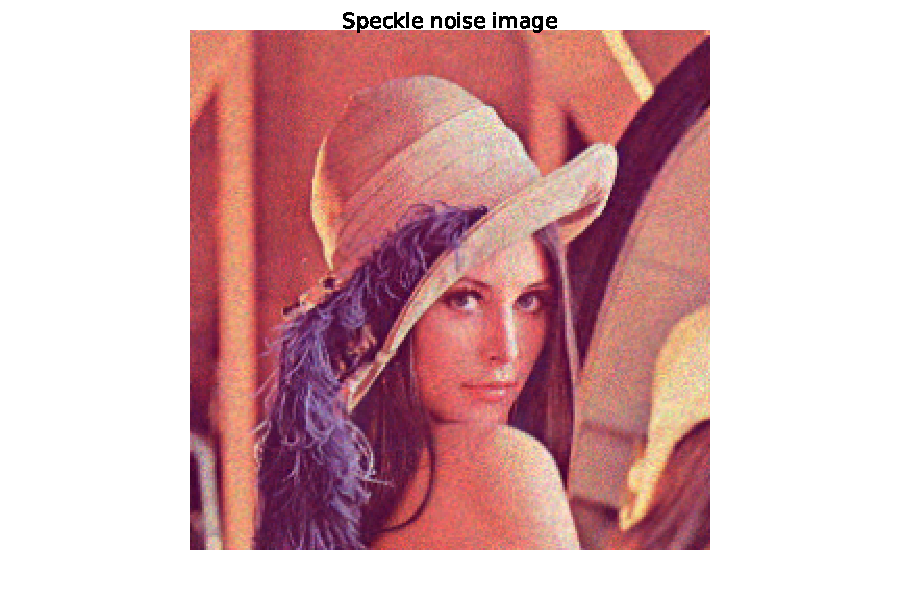
\includegraphics[width=0.24\textwidth]{figs/speckle}
  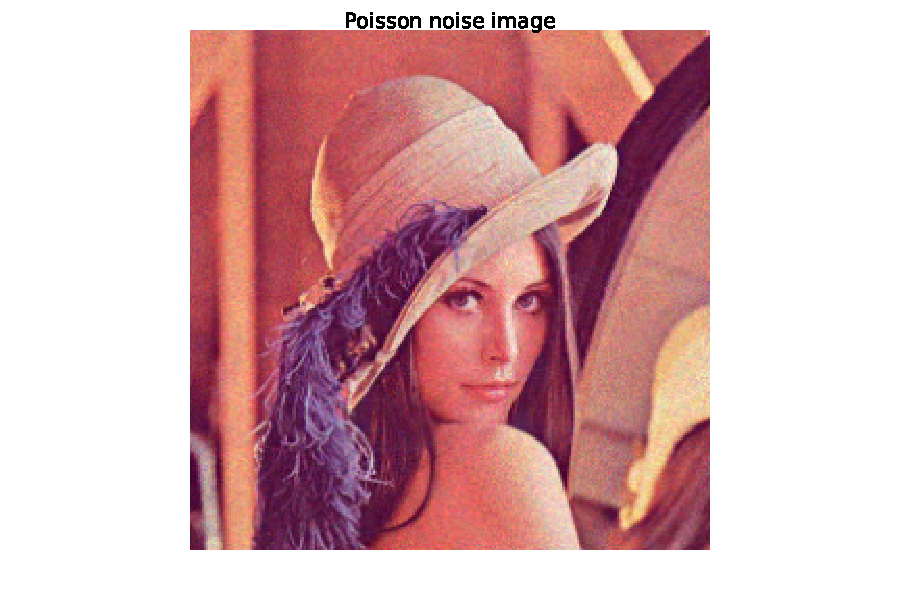
\includegraphics[width=0.24\textwidth]{figs/poisson}
  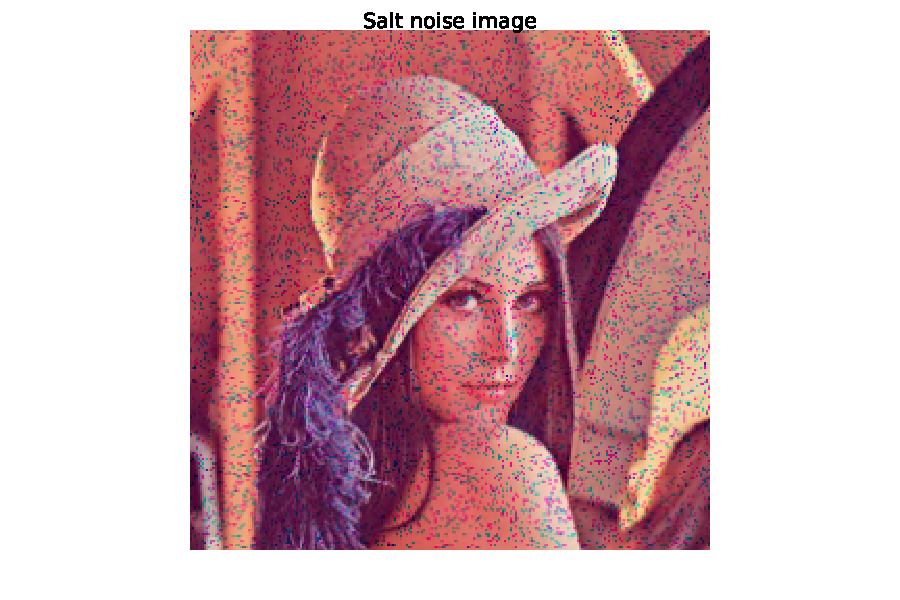
\includegraphics[width=0.24\textwidth]{figs/salt}
  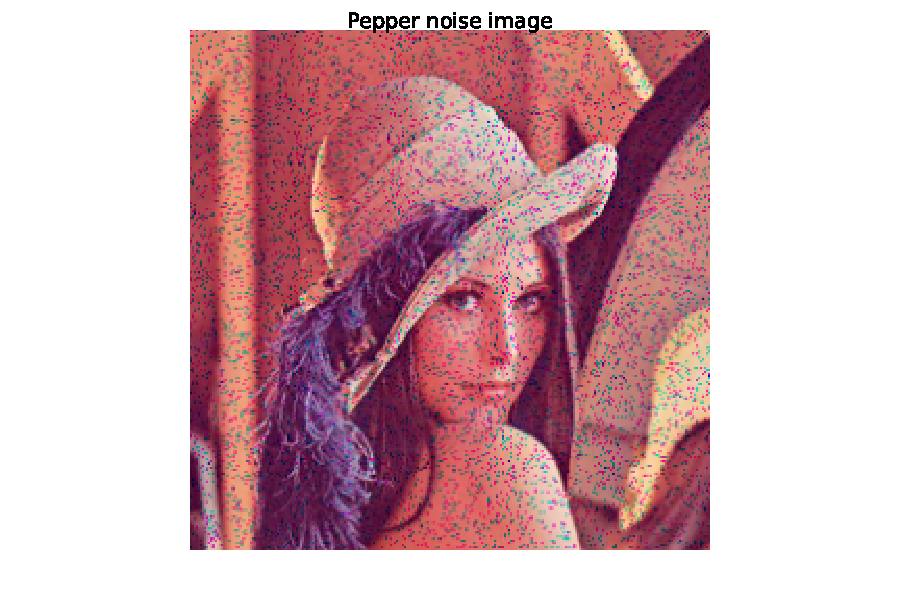
\includegraphics[width=0.24\textwidth]{figs/pepper} \\{}
  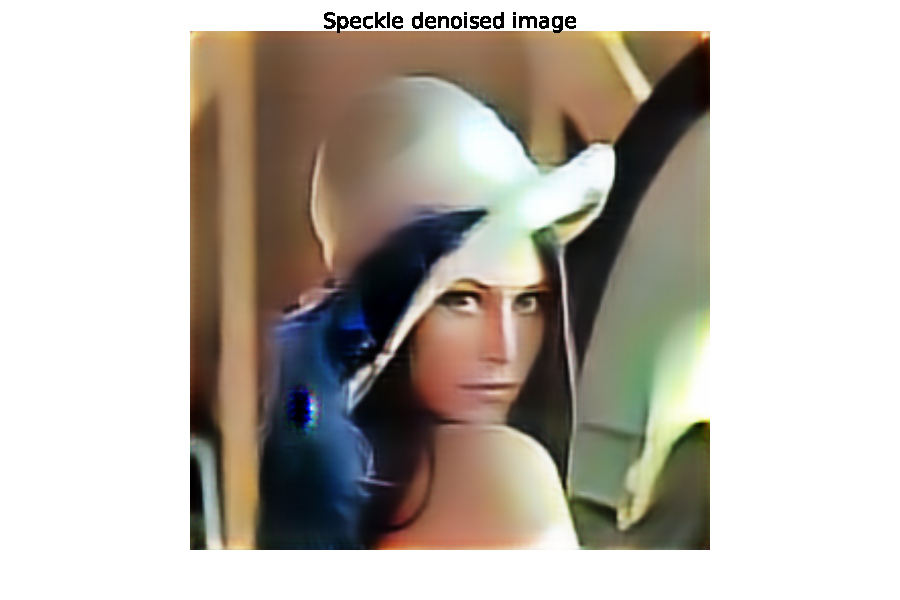
\includegraphics[trim={160pt 30pt 150pt 200pt},width=0.24\textwidth,clip]{figs/speckle_denoised}
  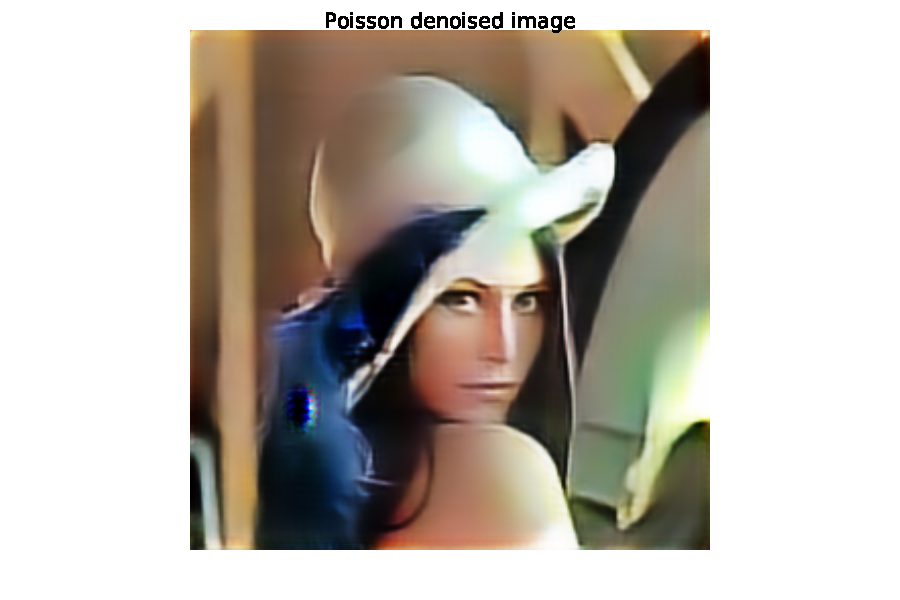
\includegraphics[trim={160pt 30pt 150pt 200pt},width=0.24\textwidth,clip]{figs/poisson_denoised}
  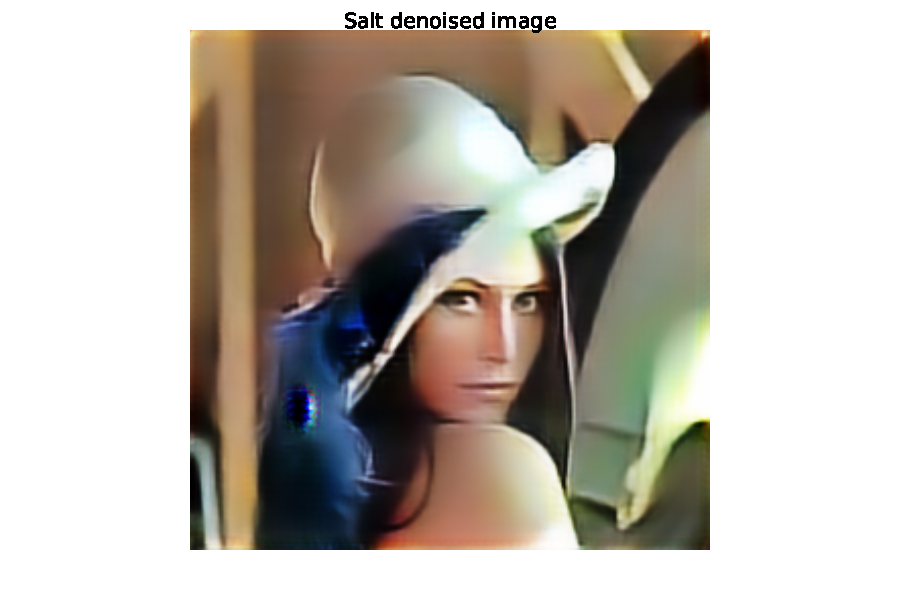
\includegraphics[trim={160pt 30pt 150pt 200pt},width=0.24\textwidth,clip]{figs/salt_denoised}
  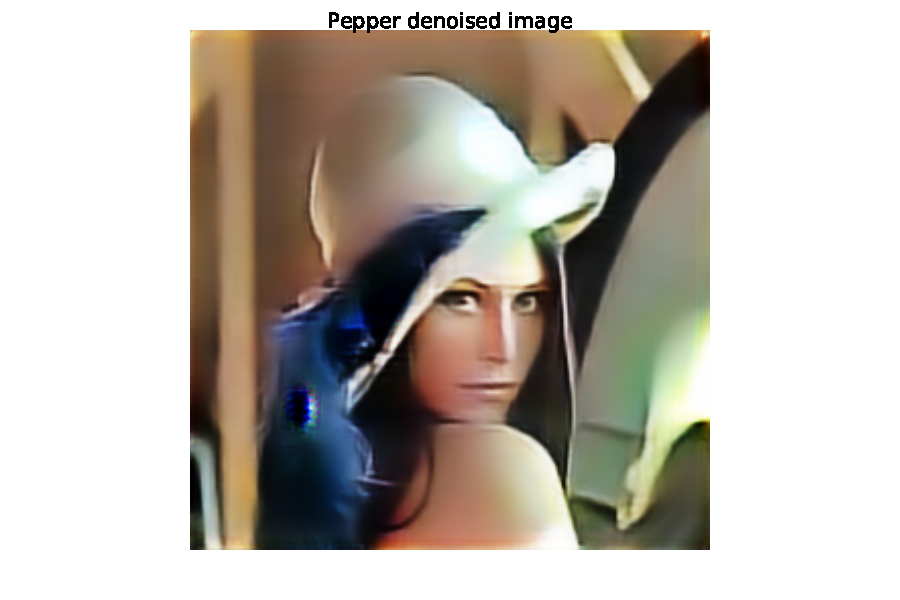
\includegraphics[trim={160pt 30pt 150pt 200pt},width=0.24\textwidth,clip]{figs/pepper_denoised} \\
    
   \caption[四种其他噪声类型的去噪比较结果图]{四种其他噪声类型的去噪性能比较图,其中变换网络仅用高斯噪声进行训练。\textbf{Up:}四种类型的噪声图像:散斑噪声,泊松分布噪声,椒盐噪声,胡椒噪声。\textbf{Down:}从相应的噪声类型中去噪输出。
   }
   \vspace{-4mm}
   \label{fig:other-type-results}
 \end{figure}
 
